\graphicspath{{Images/}}

\section{Part 0 - Environment Setup}

\textit{You will perform all your experiments in the same 50 gridworlds of size 101 × 101. You first need to generate these environments appropriate. To do so, generate a maze/corridor-like structure with a depth-first search approach by using random tie breaking. Build your 50 grid world environments with the above or a similar process of your preference and store them. You are encouraged to consider methods available online for maze generation. Provide a way to load and visualize the grid world environments you have generated.}

* NOTE: To run the program, please launch the fastTrajectoryReplanning.py python script. *

To accomplish this task, I chose to leverage the pygame library to construct a grid-like structure composed of rectangles. The code snippet provided below, found in the mazes/mazeBuilder.py file, is responsible for generating the configuration of the rectangular cells, designating them as blocked, unblocked, starting, or ending spots:


\begin{minted}{python}
import numpy as np
import os

def is_valid(x, y, grid_length):
    return 0 <= x < grid_length and 0 <= y < grid_length

def get_unvisited_neighbors(x, y, grid, visited):
    neighbors = []
    directions = [(0, 1), (0, -1), (1, 0), (-1, 0)]
    for dx, dy in directions:
        nx, ny = x + dx, y + dy
        if is_valid(nx, ny, len(grid)) and not visited[nx][ny]:
            neighbors.append((nx, ny))
    return neighbors

def generate_maze(grid_length):
    grid = np.zeros((grid_length, grid_length), dtype=int)
    visited = np.zeros((grid_length, grid_length), dtype=bool)
    stack = [(0, 0)]

    while stack:
        x, y = stack[-1]
        visited[x][y] = True
        unvisited_neighbors = get_unvisited_neighbors(x, y, grid, visited)

        if unvisited_neighbors:
            nx, ny = unvisited_neighbors[np.random.choice(len(unvisited_neighbors))]
            stack.append((nx, ny))
            grid[nx][ny] = 0 if np.random.random() < 0.7 else 1
        else:
            stack.pop()

    # Randomly select two points and mark them as 0 and -1
    start_point = np.random.choice(grid_length, size=(2,), replace=False)
    end_point = np.random.choice(grid_length, size=(2,), replace=False)

    grid[start_point[0]][start_point[1]] = 2
    print(f'Starting Point: {start_point[0]}, {start_point[1]}')
    grid[end_point[0]][end_point[1]] = -1
    print(f'Ending Point: {end_point[0]}, {end_point[1]}')

    return grid

script_dir = os.path.dirname(os.path.abspath(__file__))
for maze in range(50):
    grid_length = 101
    print(f'Maze {maze}')
    grid = generate_maze(grid_length)

    filename = os.path.join(script_dir, f'maze{maze}.txt')
    np.savetxt(filename, grid, delimiter=",", newline="\n", fmt='%i')
    

print('Done')
\end{minted}
The \texttt{mazeBuilder.py} script generates maze-like structures using a depth-first search approach with random tie-breaking. Here is a breakdown of the key functions:

\begin{enumerate}
    \item \texttt{is\_valid(x, y, grid\_length)}: Checks if coordinates \((x, y)\) are within the bounds of the grid (\texttt{grid\_length x grid\_length}).
    
    \item \texttt{get\_unvisited\_neighbors(x, y, grid, visited)}: Returns a list of unvisited neighboring positions of \((x, y)\) on the grid, considering the \texttt{visited} matrix.
    
    \item \texttt{generate\_maze(grid\_length)}: Initializes a grid and a \texttt{visited} matrix. Performs depth-first search using a stack to navigate through the grid. Randomly chooses unvisited neighbors, marks paths based on a random probability, and designates starting (2) and ending (-1) points.
\end{enumerate}

The script iterates through 50 mazes, generates mazes, and saves them to text files (\texttt{maze0.txt}, \texttt{maze1.txt}, etc.).
These text files are saved within the mazes folder. I then use these text files within the main source code to generate the pygame interface.

The source code loads a specified maze, visualizes it using \texttt{pygame}, and allows user interaction. The user can enter a maze number (0 to 49), and the corresponding maze is loaded and displayed. Colors represent different elements: light green for open paths, purple for walls, red for the starting point, and orange for the ending point. The \texttt{pygame} window enables the user to close the application or interact with the maze using key events (handled by \texttt{handle\_key\_event} function which I plan to implement so that when a user presses a button, it either generates a path or cleans the board). Here's the example of running the program and loading a maze. 

 % % % % % % % % % % % % % % % % % % %
% % % % %  SAMPLE IMAGE   % % % % % %
% % % % % % % % % % % % % % % % % % %

\begin{figure}[h]
    \centering
    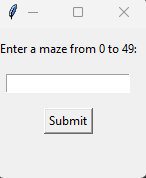
\includegraphics[width=.25\linewidth]{imgs/maze_prompt.png}
    \caption{Prompting for an Maze Number}
    \label{fig:my_label}
\end{figure}
\begin{figure}[h]
    \centering
    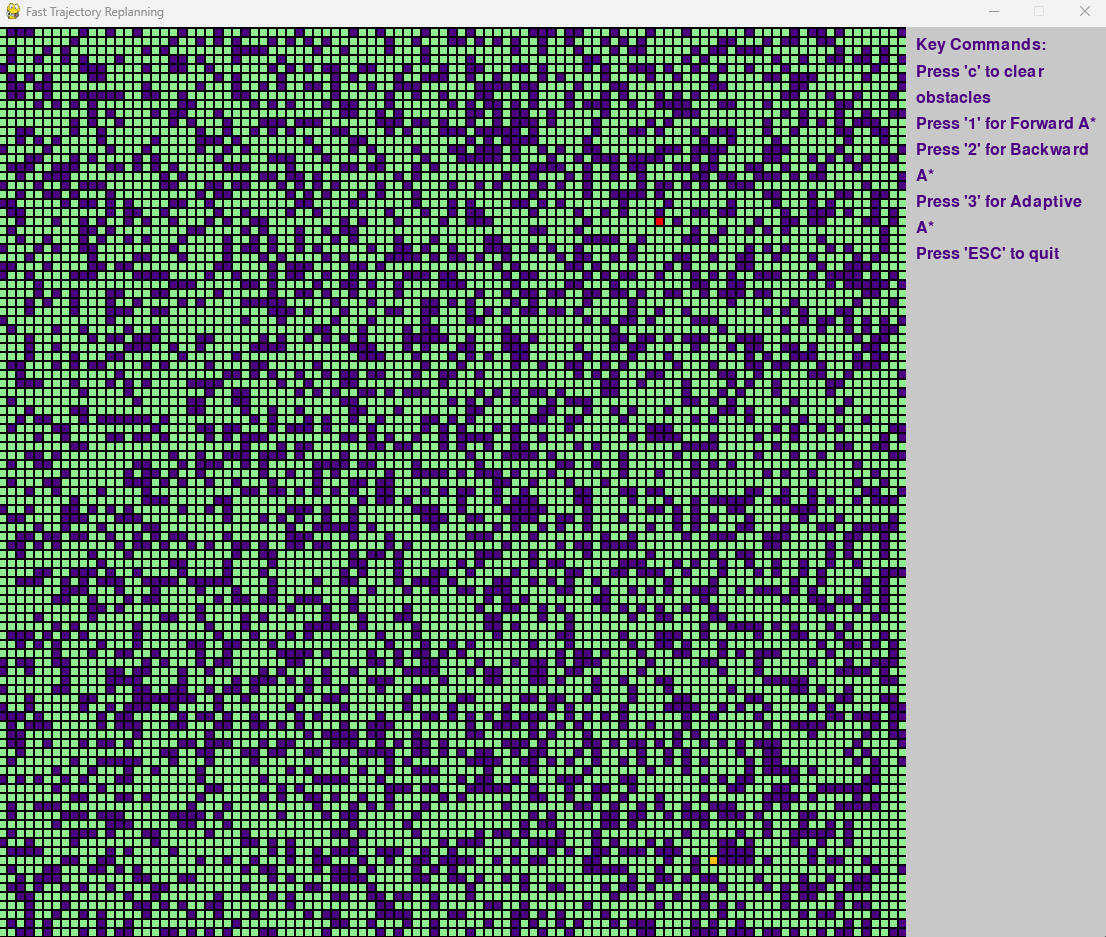
\includegraphics[width=.85\linewidth]{imgs/FRT.png}
    \caption{Visualization of the Maze}
    \label{fig:my_label}
\end{figure}
% % % % % % % % % % % % % % % % % % % % %
% % % % %  SAMPLE EQUATIONS   % % % % % %
% % % % % % % % % % % % % % % % % % % % %


